% $Id: $
\documentclass[a4paper, 10pt]{article}
% reduced margins
\usepackage{fullpage}
\usepackage[authoryear,round]{natbib}
% spacing		
\usepackage{setspace}
% page headings
\usepackage{fancyhdr}
%\usepackage{lscape}

\let\subequations\relax

\usepackage{pdflscape}

\usepackage[acronym,toc]{glossaries} % nomain, if you define glossaries in a file, and you use \include{INP-00-glossary}
\input{glossary.tex}
\makeglossaries

\usepackage{subfigure} 
\usepackage[margin=1.0in]{geometry}
\usepackage{url}
%\usepackage{subeqn}
\usepackage{multirow}
\usepackage{booktabs}

\setlength{\headheight}{15.2pt}
\pagestyle{fancy}

\usepackage{graphicx}
\usepackage{color}
\usepackage{hyperref}
\usepackage{url}
\hypersetup{colorlinks, urlcolor=darkblue}


\usepackage{lscape}
% figs to be 75% of test width
\setkeys{Gin}{width=0.75\textwidth}


\newcommand{\mathgloss}[2]{
 \newglossaryentry{#1}{name={#1},description={#2}}
 \gls{#1} = #2
}
\newcommand{\ds}{\displaystyle}
\newcommand{\eps}{\epsilon}
\newcommand{\veps}{\varepsilon}
\newcommand{\wh}{\widehat}

%
\renewcommand{\abstractname}{\large SUMMARY}
%
\newcommand{\Keywords}[1]{\begin{center}\par\noindent{{\em KEYWORDS\/}: #1}\end{center}}
%
\makeatletter
\renewcommand{\subsubsection}{\@startsection{subsubsection}{3}{\z@}%
 {-1.25ex\@plus -1ex \@minus -.2ex}%
 {1.5ex \@plus .2ex}%
 {\normalfont\slshape}}
\renewcommand{\subsection}{\@startsection{subsection}{2}{\z@}%
 {-3.25ex\@plus -1ex \@minus -.2ex}%
 {1.5ex \@plus .2ex}%
 {\normalfont\bfseries\slshape}}
\renewcommand{\section}{\@startsection{section}{1}{\z@}%
 {-5.25ex\@plus -1ex \@minus -.2ex}%
 {1.5ex \@plus .2ex}%
 {\normalfont\bfseries}}
\makeatother
%
\renewcommand\thesection{\arabic{section}.}
\renewcommand\thesubsection{\thesection\arabic{subsection}}
\renewcommand\thesubsubsection{\thesubsection\arabic{subsubsection}}
%
\renewcommand{\headrulewidth}{0pt}

\usepackage{listings}

\newenvironment{mylisting}
{\begin{list}{}{\setlength{\leftmargin}{1em}}\item\scriptsize\bfseries}
{\end{list}}

\newenvironment{mytinylisting}
{\begin{list}{}{\setlength{\leftmargin}{1em}}\item\tiny\bfseries}
{\end{list}}

\usepackage{listings}

\definecolor{darkblue}{rgb}{0,0,0.5}
\definecolor{shadecolor}{rgb}{1,1,0.95}
\definecolor{shade}{rgb}{1,1,0.95}


\lstset{ %
language=R, % the language of the code
basicstyle=\footnotesize, % the size of the fonts that are used for the code
numbers=left, % where to put the line-numbers
numberstyle=\footnotesize, % the size of the fonts that are used for the line-numbers
stepnumber=1	00, % the step between two line-numbers. If it's 1, each line 
 % will be numbered
numbersep=5pt, % how far the line-numbers are from the code
backgroundcolor=\color{shade}, % choose the background color. You must add \usepackage{color}
showspaces=false, % show spaces adding particular underscores
showstringspaces=false, % underline spaces within strings
showtabs=false, % show tabs within strings adding particular underscores
frame=single, % adds a frame around the code
tabsize=2, % sets default tabsize to 2 spaces
captionpos=b, % sets the caption-position to bottom
breaklines=true, % sets automatic line breaking
breakatwhitespace=false, % sets if automatic breaks should only happen at whitespace
title=\lstname, % show the filename of files included with \lstinputlisting;
 % also try caption instead of title
escapeinside={\%*}{*)}, % if you want to add a comment within your code
morekeywords={*,...} % if you want to add more keywords to the set
}

%
\title{An Example Management Strategy Evaluation Of A Model Free Harvest Control Rule.}
%
\author{Laurence T. Kell\footnote{ICCAT Secretariat, C/Coraz\'{o}n de Mar\'{\i}a, 8. 28002 Madrid, Spain; ~Laurie.Kell@iccat.int; ~Phone: +34 914 165 600 ~Fax: +34 914 152 612.}~,
        Richard Hillary\footnote{CSIRO, Australia}~,\\
        Jean Marc Fromentin\footnote{IFREMER - UMR EME 212, Av. Jean Monnet, 34200 S\`ete, France.}~and
        Sylvain Bonhommeau\footnotemark[3] }
\date{}
%


\begin{document}

\onehalfspacing
\lhead{\normalsize\textsf{SCRS/2014/36}}
\rhead{}

\maketitle
% gets headers on title page ...
\thispagestyle{fancy}
% ... but not on others
\pagestyle{empty}

%
\begin{abstract}


\end{abstract}

\Keywords{Bluefin, Harvest Control Rule, FLR, Management Procedure, Management Strategy Evaluation, Model Free}

 
\newpage
\tableofcontents
\newpage
 
 
\section[Introduction]{Introduction}

A \gls{HCR} relates the recommended catch, or other fishery control 
measure, to the current value of selected control variables. A HCR may be empirical where
control variables are directly measurable quantities (e.g., catch rate, size 
composition, tag recovery rate, survey estimates of abundance or species 
composition) or model based on using a statistical procedure (i.e. an estimator) 
that provides information on resource status and productivity from past resource 
monitoring data.

An empirical HCR has been adopted for \gls{SBT} which sets the \gls{TAC} 
using data solely from a fisheries dependent \gls{cpue} 
index of adult abundance and a fisheries independent aerial survey of juveniles. The HCR is based on year-to-year 
changes and in the indices. Before the HCR can be implemented appropriate 
reference levels (e.g. based on historical catch, effort, CPUE and/or surveys) must be selected and the parameters tuned 
to meet management objectives using \gls{MSE}. The HCR is therefore evaluated as part of a \gls{MP}, i.e. the combination of pre-defined data, 
together with an algorithm to which the data are input to provide a value for a TAC or effort control measure.

We first describe the empirical (i.e model free) HCRs used by CCSBT and then conduct an MSE for Atlantic bluefin
tuna. 

\section{Management Strategy Evaluation}

Data for use in the \gls{MP} are sampled from the \gls{OM} via the \gls{oem}. Where the \gls{OM} 
is a mathematical–statistical model used to describe the actual resource dynamics in simulation trials and to generate 
resource monitoring data when projecting forward. The \gls{OM} generates fishery-dependent and/or fishery-independent resource 
monitoring data for input to the \gls{MP}. The aim of an \gls{MSE} is to demonstrate through simulation 
trials the robust performance of \gls{feedback control} rules in the presence of uncertainties. 

\subsection{Operating Model}

The \gls{OM} is based on the East Atlantic and Mediterranean BFT assessment \cite{kell2012bftkobe}. 
The assessment was conducted using \gls{vpa} in 2012 for two assumed historical catch levels and three future recruitment
(i.e. six scenarios were considered). The two levels of catch corresponded to the \textbf{reported} and \textbf{inflated} 
levels; in the latter case catches were raised to 50,000 tonnes from 1998 to 2006 and to 61,000 tonnes in 2007 to allow
for the possibility of actual catches being greater than those reported. Recruitment had varied over the
historic period \cite{kell2014chicken} and so the three 
recruitment scenarios  \textbf{low}, \textbf{high}  and \textit{medium} were based on recruitment over different 
historical periods. 

\subsubsection{Scenarios}

The scenarios are given in \textbf{Table} \ref{tab:om}.

\subsection{Management Procedure}

The MPs are based on the model free HCR developed by \gls{CCSBT}. The TAC is an average of candidate TACs obtained from two harvest control rules. Here we
run the two HCRs separately in order to compare their performance \citep{hillary2013sbthcr}.

\subsubsection{Harvest Control Rule I}

The first HCR is based on a single index i.e.

\begin{equation}
            \ds TAC^1_{y+1}=TAC_y\times \left\{\begin{array}{rcl}\ds{1-k_1|\lambda|^{\gamma}} & \mbox{for} & \lambda<0\\[0.35cm]
\ds{1+k_2\lambda} & \mbox{for} & \lambda\geq 0 
    \end{array}\right.
\end{equation}
        

 where $\lambda$ is the slope in the regression of $\ln B_y$ against year for the most recent $n$ years,  
 $k_1$ and $k_2$ are \textit{gain} parameters.

giving 4 tunable parameters (\textbf{Table} \ref{tab1})


\subsubsection{Harvest Control Rule II}

The second HCR uses both a biomass and a juvenile index i.e.

\begin{equation} 
 \begin{align*}
 \ds TAC_{y+1} &= 0.5\times\left(TAC_y+C^{\rm targ}_y\Delta^R_y\right),\\
 \end{align*}
  \end{equation}

and

 \begin{equation}
       \begin{align*}
            \ds TAC^2_{y+1} &= 0.5\times\left(TAC_y+C^{\rm targ}_y\Delta^R_y\right),\\
                \ds C^{\rm targ}_y &= \left\{\begin{array}{rcl}\ds{\delta \left[\frac{B_{y}}{B^*}\right]^{1-\veps_b}} & \mbox{for} & B_{y}\geq B^*\\[0.35cm]
\ds{\delta \left[\frac{B_{y}}{B^*}\right]^{1+\veps_b}} & \mbox{for} & B_{y}<B^*
    \end{array}\right.,\\
\ds \Delta^R_y &= \left\{\begin{array}{rcl}\ds{\left[\frac{\bar{R}}{\mathcal{R}}\right]^{1-\veps_r}} & \mbox{for} & \bar{R}\geq\mathcal{R}\\[0.35cm]
\ds{\left[\frac{\bar{R}}{\mathcal{R}}\right]^{1+\veps_r}} & \mbox{for} & \bar{R}<\mathcal{R}
\end{array}\right.
        \end{align*}
  \end{equation}

 where $\delta$ is the \textit{target} catch; $B^*$ the \textit{target} CPUE (i.e. the mean observed CPUE corresponding to some 
 multiple of a biomass reference point such as $B_0$ or $M_{MSY}$) and 
$\bar{R}$ is the average recent juvenile biomass i.e.

\begin{equation}
 \ds \bar{R}=\frac{1}{\tau_R}\sum\limits_{i=y-\tau_R+1}^{y}R_i,
 \end{equation}

 
$\mathcal{R}$ is a ``limit'' level derived from the mean recruitment over a reference period; \\
while $\veps_\bullet\in[0,1]$ actions asymmetry so that increases in TAC do not occur at the same level as decreases.

There are therefore 5 tunable parameters, \textbf{Table} \ref{tab2}

In our example we use reference periods to set $\delta$ as well as $\mathcal{R}$. 

The MP operates every three years, i.e. 

\begin{enumerate}
 \item In year $t$ historical data up to and including $t-1$ are sampled from the \gls{OM} by the \gls{oem}
 \item These data are then used by the \gls{MP} to set a quota for 3 years starting in years $t+1$. 
 \item repeat step 1 for year $t+4$
\end{enumerate}


\subsection{Observation Error Model}

A simple \gls{oem} was constructed to generate two unbiased abundance indices corresponding to the adult biomass and numbers of recruits.
A log normal random error of 30\% was added to these time series.

\section{Results and Discussion}

Catch, fishing mortality, recruitment and SSB are summarised in \textbf{Figure} \ref{fig:1} for the 2 HCRs and 6 OM Scenarios.
Worm plots (i.e. single iterations) for yield, fishing mortality, recruits and SSB are shown in \textbf{Figures} \ref{fig:2}, \ref{fig:3}, \ref{fig:4} and \ref{fig:5}. 

The HCR parameters were not tuned to achieve the best performance 
but ran with default values. This was because the intention of the study was to provide a simple example of model 
free HCRs. 

To conduct a full MSE involves a number of steps \citep[][]{punt2007developing} i.e.

\begin{itemize}
 \item identification of management objectives and mapping these to performance measures in order to quantify how well they have been achieved.
 \item selection of hypotheses about system dynamics.
 \item conditioning of OMs on data and knowledge and possible rejecting and weighting the different hypotheses.
 \item identifying candidate management strategies and coding these up as MPs %(i.e.the combination of pre-defined data, together with an algorithm to which such data are input to set control measures).
 \item projecting the OMs forward using the MPs as feedback control procedures; and
 \item agreeing the MPs that best meet  management objectives.
\end{itemize}

The next steps will be to compare the performance of empirical HCRs to model based ones, such as those documented in \cite{kell2013mpalbn,
kell2013msealbn}. This will require a number of scenarios to be considered that reflect the uncertainty about 
resource dynamics \citep[e.g.][]{fromentin2014spectre,leach2014elicit,kell2014bftuncert,kell2014chicken}.

\newpage\clearpage
\bibliography{refs} 
\bibliographystyle{abbrvnat} 

\newpage\clearpage\section{Tables}

\begin{table}[ht]
\begin{center}
\begin{tabular}{|cc|}
\hline
Parameter & default\\
\hline\hline
$k_1$ & 1.5\\
$k_2$ & 3\\
$\gamma$ & 1\\
$n$ & -\\
\hline
\end{tabular}
\end{center}
\caption{HCR 1 tunable parameters}
\label{tab1}
\end{table}

\begin{table}[ht]
\begin{center}
\begin{tabular}{|cc|}
\hline
Parameter & BP\\
\hline\hline
$\veps_b$ & 0.25\\
$\veps_r$ & 0.75\\
$\delta$ & - \\
$\tau_B$ & 7\\
$B^*$ & -\\
$\tau_r$ & 5\\
\hline
\end{tabular}
\end{center}
\caption{HCR 2 tunable parameters}
\label{tab2}
\end{table}

\begin{table}
\begin{center}
\label{tab:datasumm}
\begin{tabular}{|cccc|}
\hline
{\tiny Factor} & {\tiny Levels} & {\tiny $\Sigma N$} & {\tiny Values} \\
\hline\hline
{\tiny Historic Catch} 	        & {\tiny 2}   & {\tiny  2}  	& {\tiny  Reported, Inflated}          \\
{\tiny Recruitment} 		& {\tiny 2}   & {\tiny  4}  	& {\tiny  Low,Medium,High}  	       \\
{\tiny HCR} 	   	        & {\tiny 2}   & {\tiny  8} 	& {\tiny  $1$,$2$} 	       \\
\hline
\end{tabular}
\end{center}
\caption{OM options}
\label{tab:om}
\end{table}

\newpage\clearpage

\begin{landscape}
\section{Figures}
\begin{figure}[htbp]
\centering
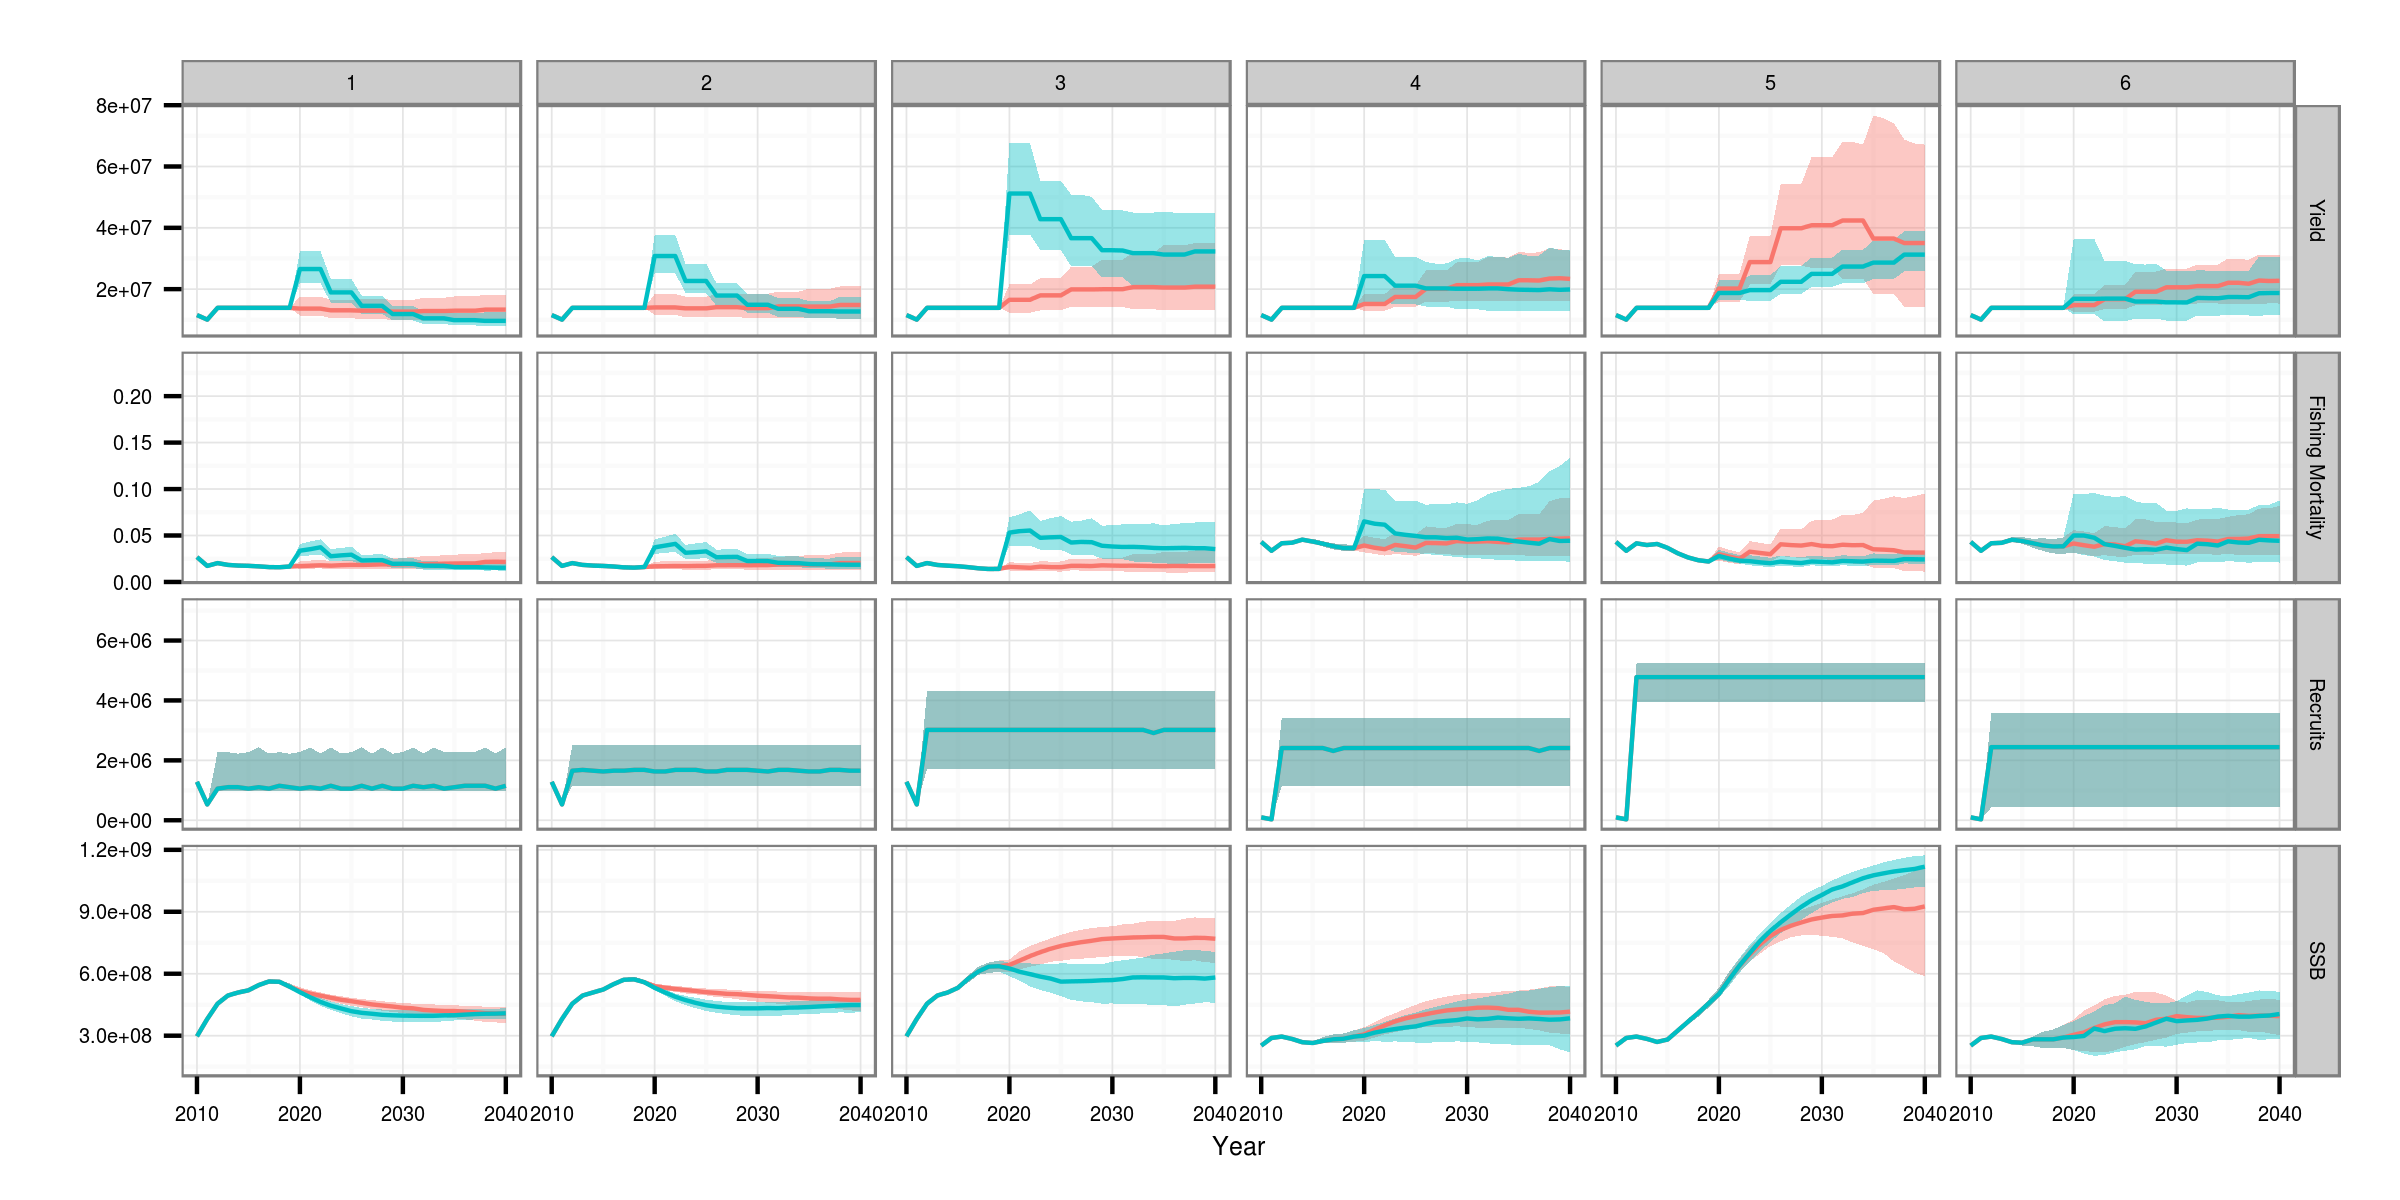
\includegraphics[width=8in]{ts.png}
\caption{Inter-quartiles (shaded area) and medians (lines) for time series of catch, SSB, recruits and fishing mortality for the 2 HCRs (colour) and 
OM Scenario (col).}
\label{fig:1}
\end{figure}
\end{landscape}

\begin{figure}[htbp]
\centering
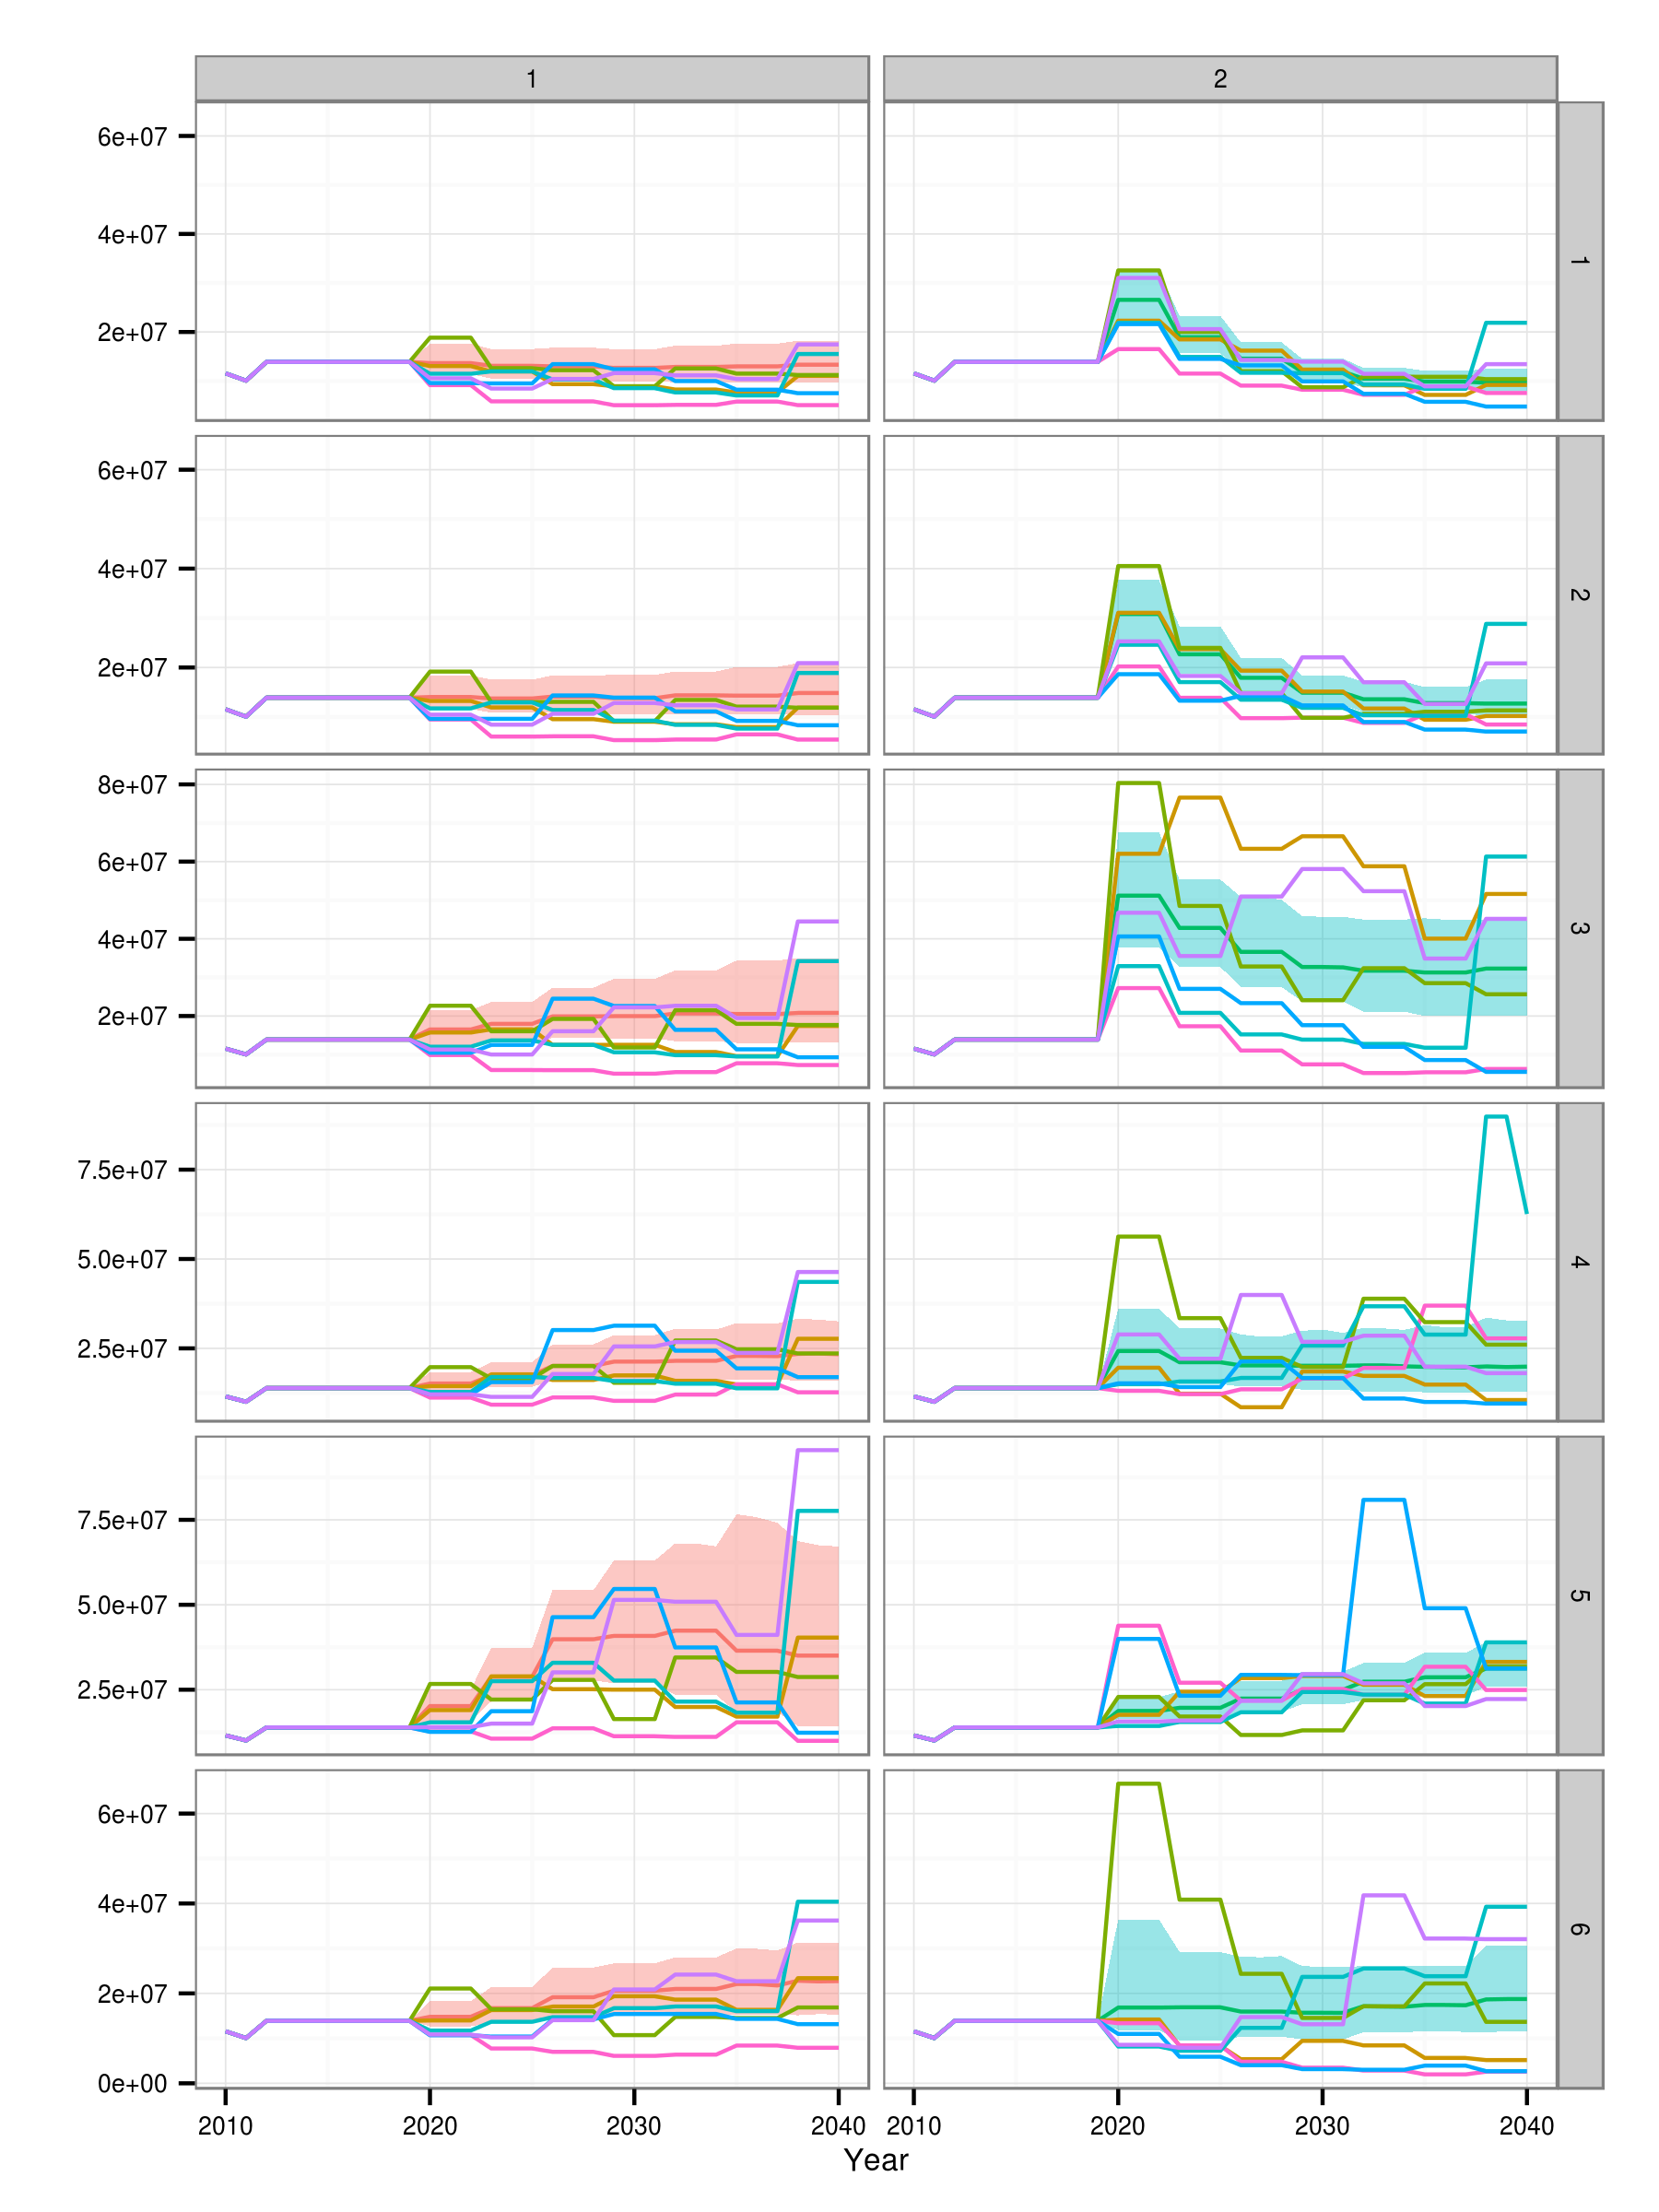
\includegraphics[width=6in]{iY.png}
\caption{Worm plots for catch by HCR (row) and OM Scenario (col).}
\label{fig:5}
\end{figure}

\begin{figure}[htbp]
\centering
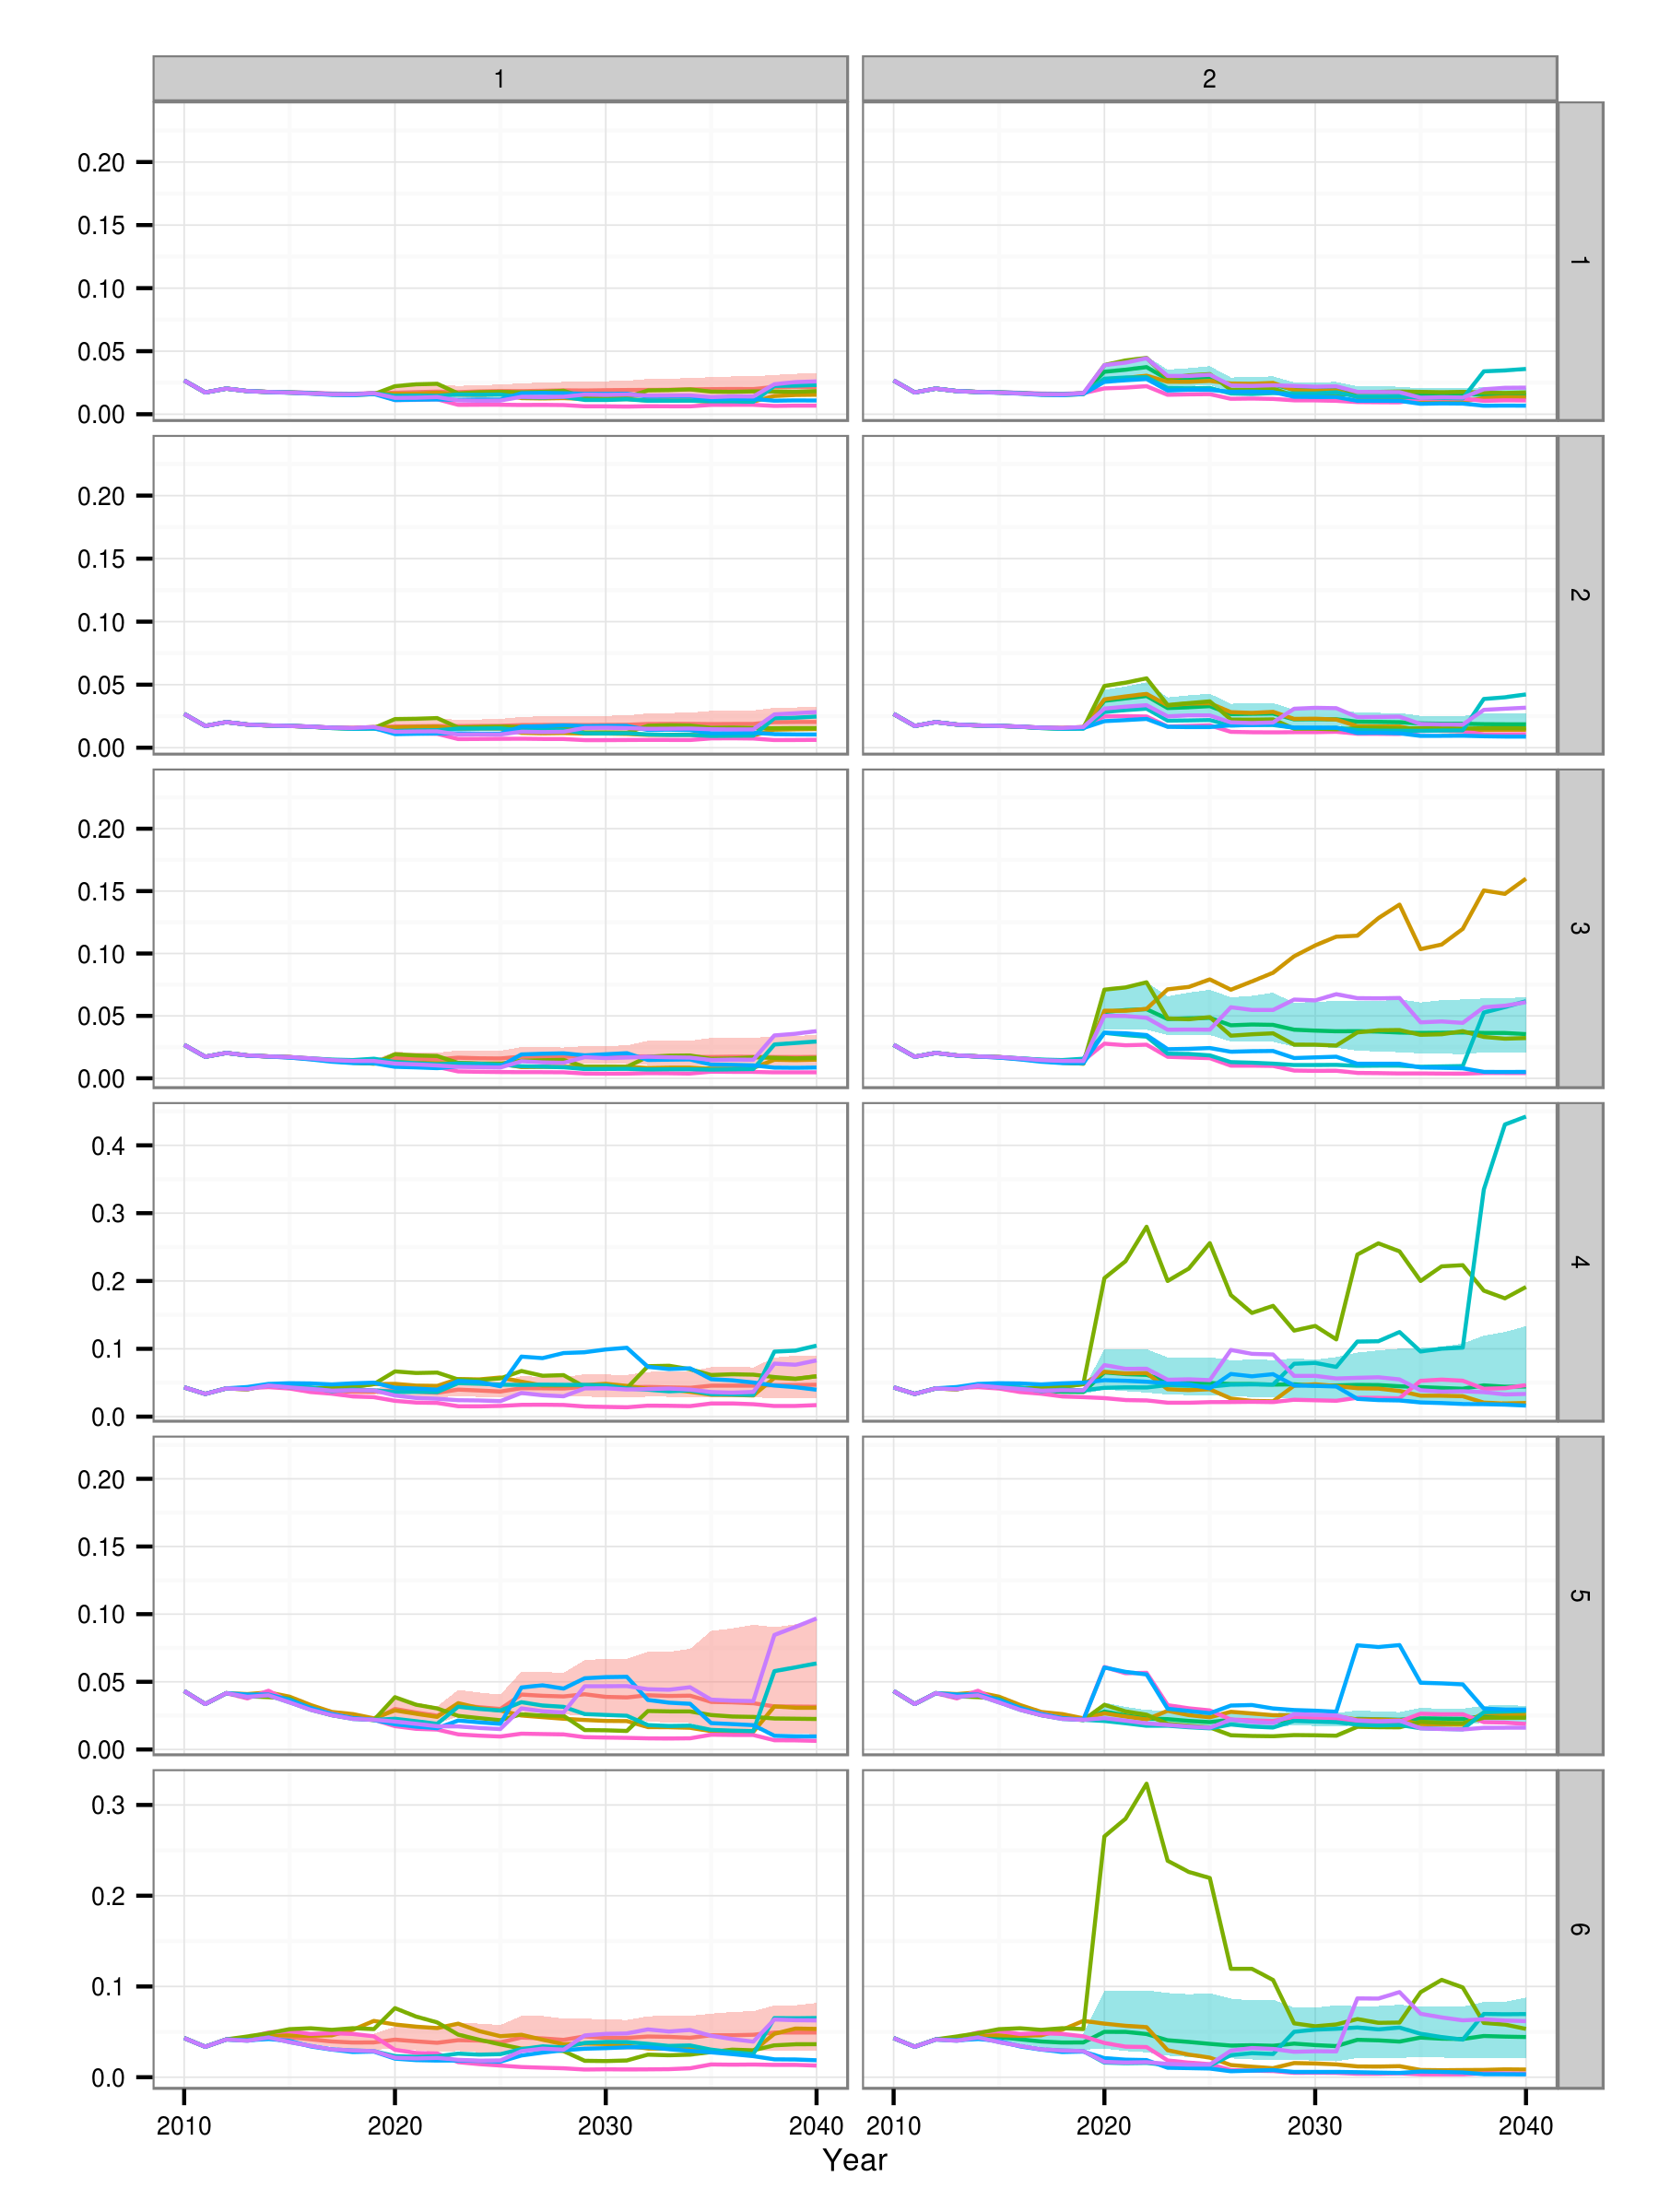
\includegraphics[width=6in]{iF.png}
\caption{Worm plots for F by HCR (row) and OM Scenario (col).}
\label{fig:4}
\end{figure}

\begin{figure}[htbp]
\centering
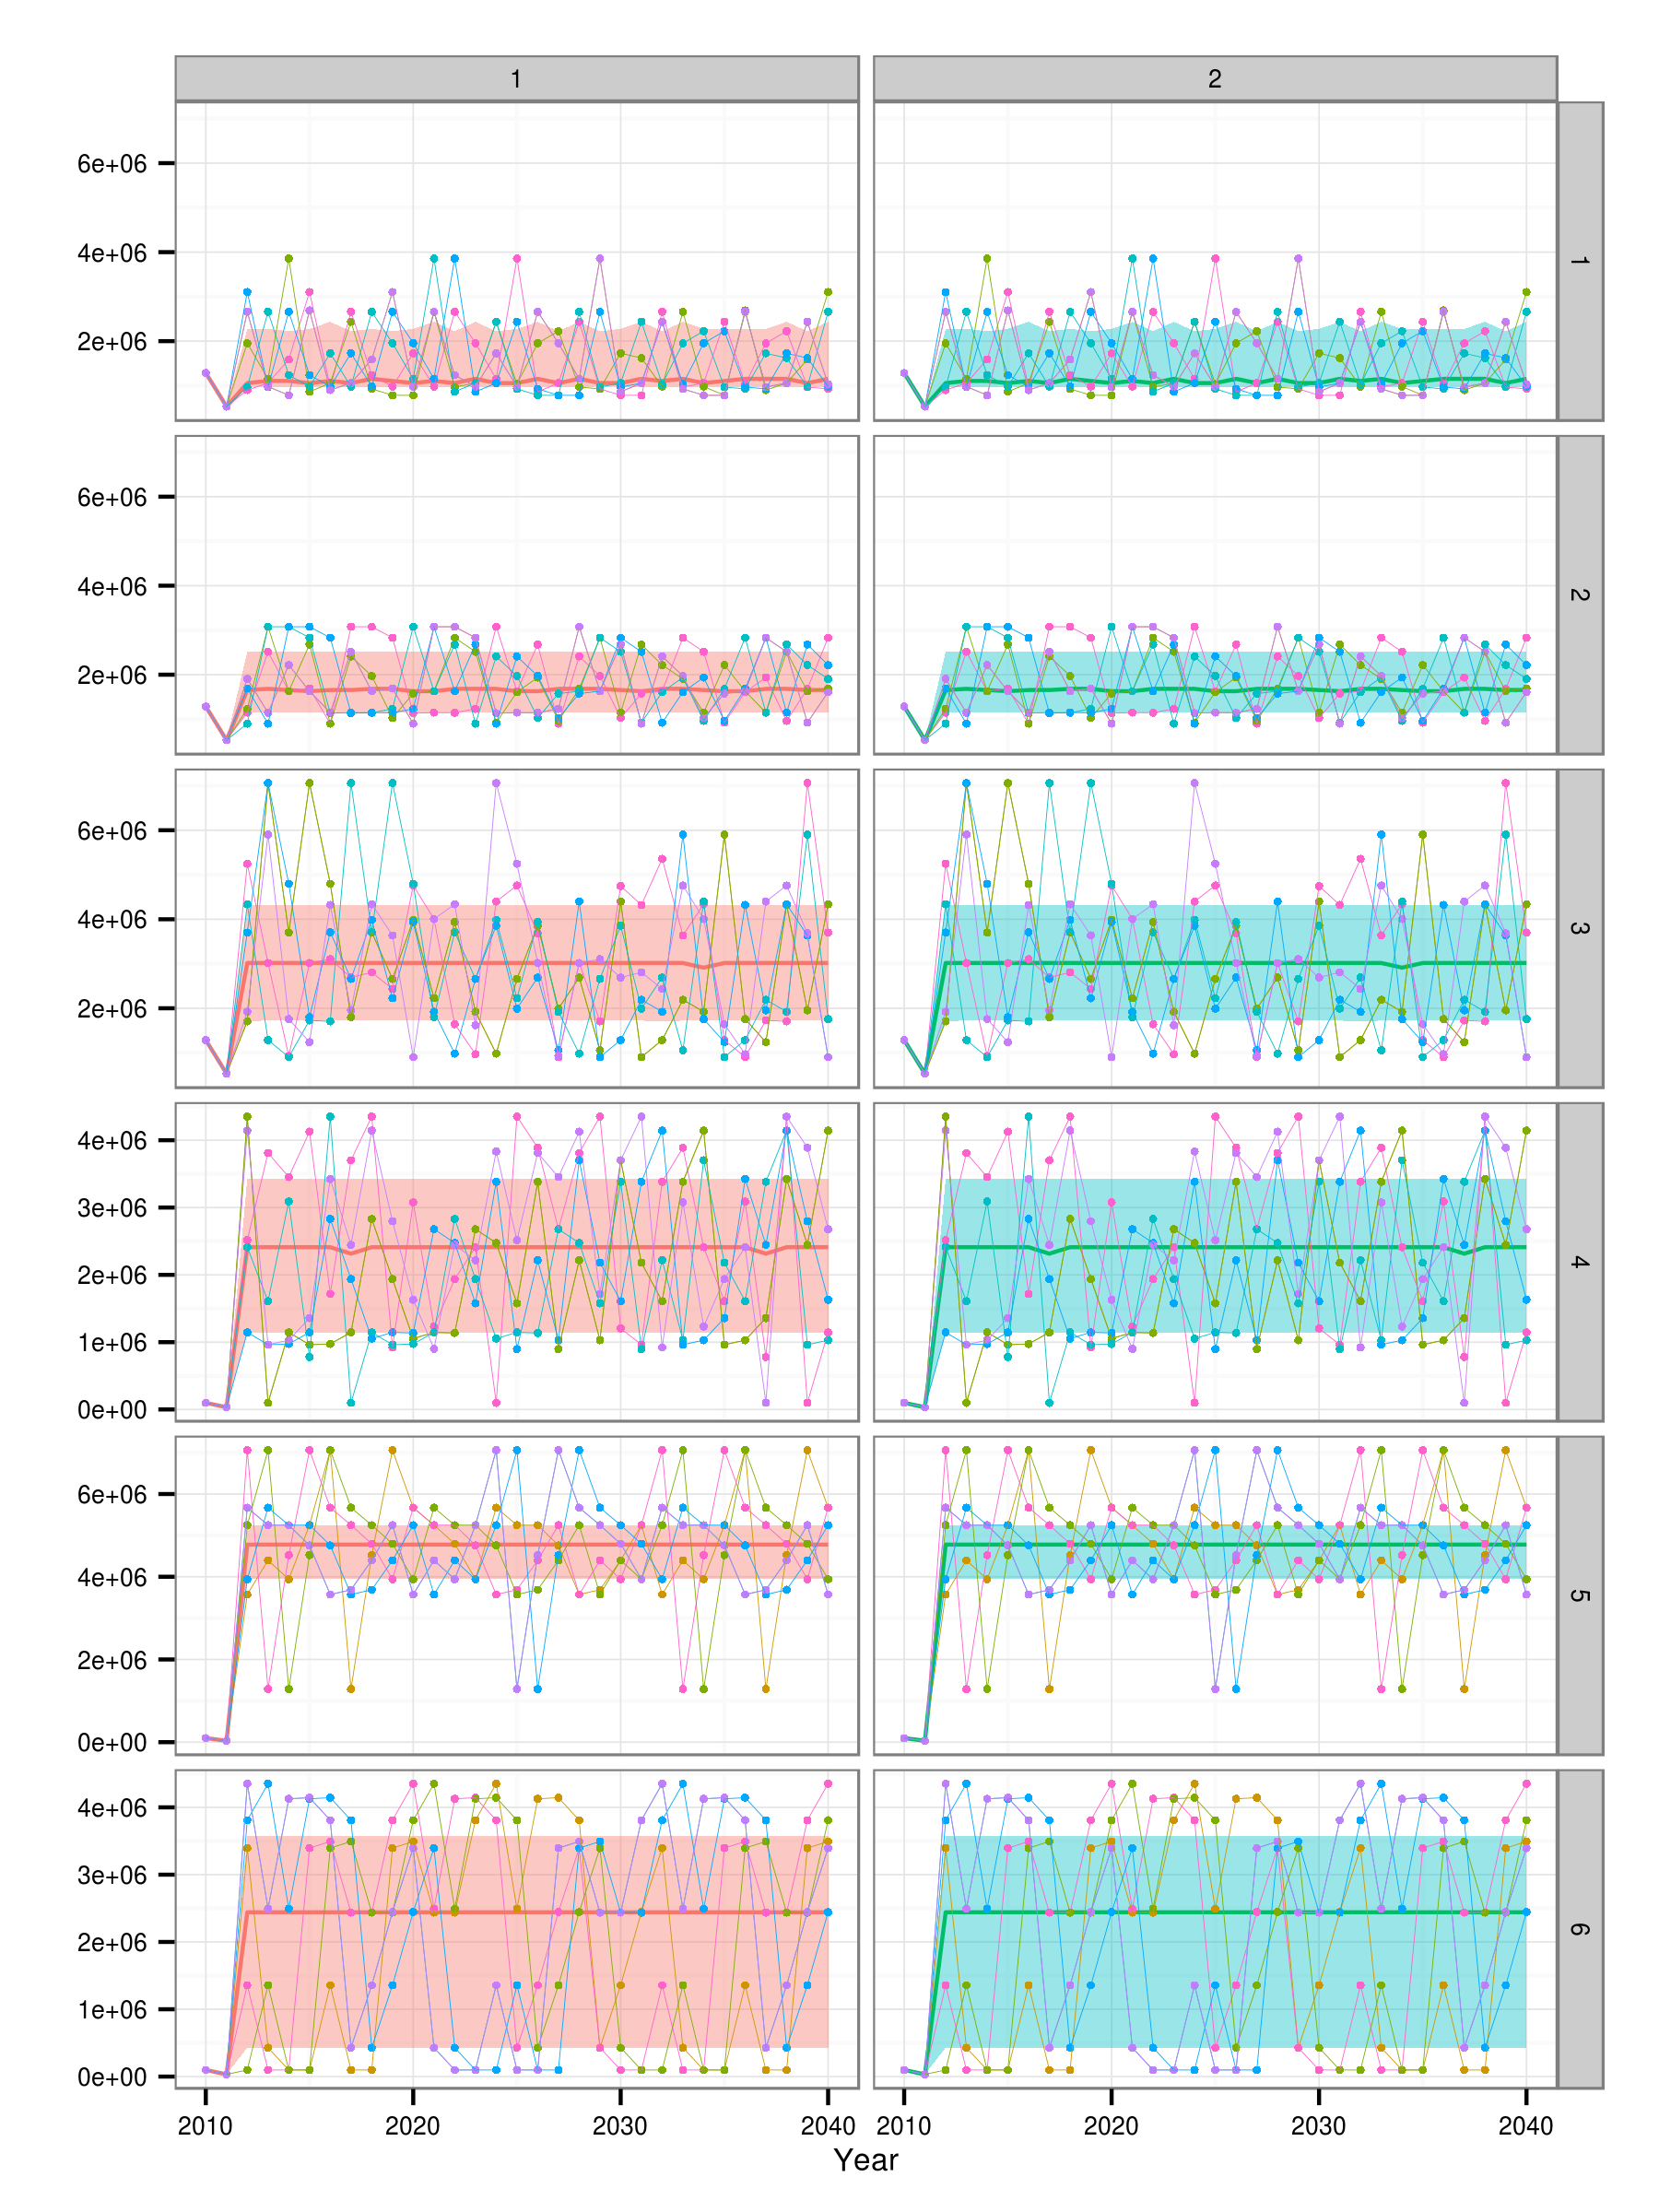
\includegraphics[width=6in]{iR.png}
\caption{Worm plots for recruits by HCR (row) and OM Scenario (col).}
\label{fig:3}
\end{figure}

\begin{figure}[htbp]
\centering
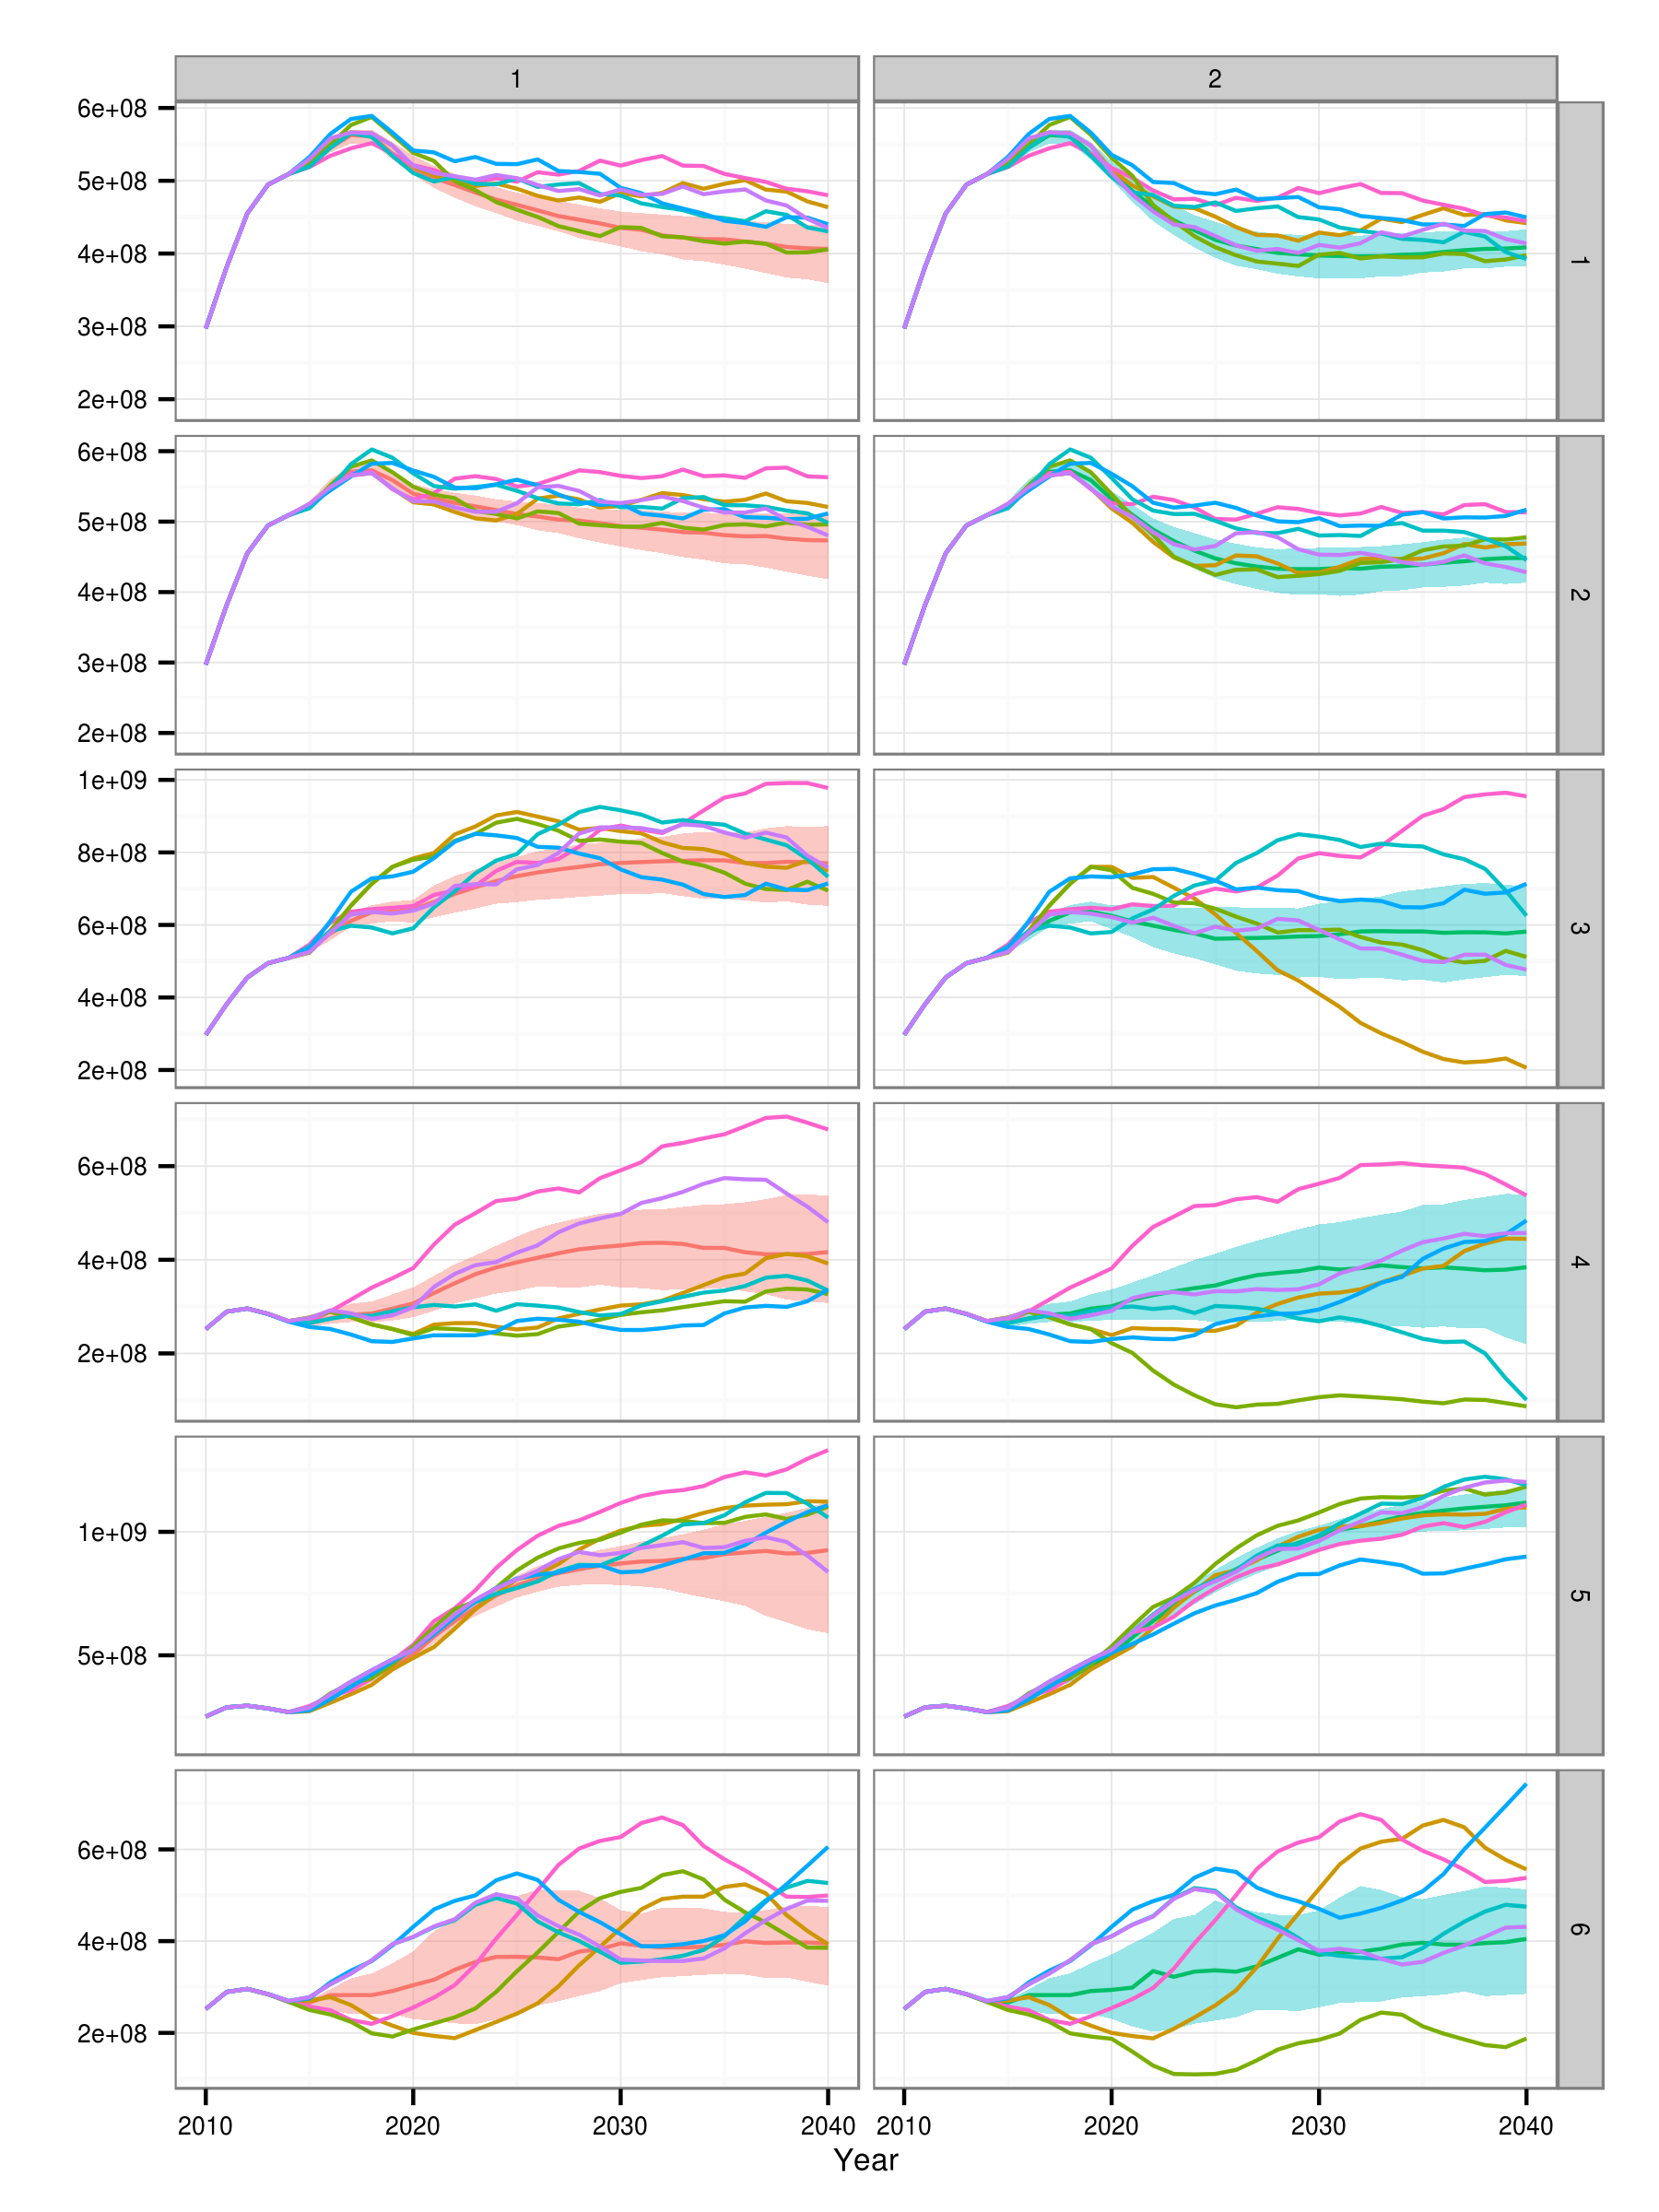
\includegraphics[width=6in]{iS.png}
\caption{Worm plots for SSB by HCR (row) and OM Scenario (col).}
\label{fig:2}
\end{figure}

\end{document}


\printglossary




\subsubsection{ICCAT}

The HCR bsing evaluated by ICCAT for \gls{alb} and \gls{swo} is shown in figure~\ref{fig:hcr} as part of a phase plot; the orange line sets the harvest rate (y-axis) depending on
the estimated stock biomass (x-axis). The black line is the replacement line, i.e. for a given stock biomass a harvest rate above the
black line will cause the stock to decline and a harvest rate below the line will cause the stock to increase. For a given target harvest rate
(i.e. the horizontal part of the HCR) the target biomass is given by the intersection of the two lines. If the stock declines below the
break point (i.e. a trigger biomass or threshold biomass reference point) the harvest rate is reduced progressively to a minimum level of 
harvest rate at a biomass level equal to the \gls{lrp}.

The corresponding algorithm is 

 \begin{equation}
 \ds F_{y+1}=
 \left\{\begin{array}{lcl}\ds F_{Target}    & \mbox{if} & B_y \geq \alpha B_{MSY} \\[0.35cm]                      
                          \ds{F_{Lim}}      & \mbox{if} & B_y \leq \beta B_{MSY}  \\[0.35cm]     
                          \ds{F_{Lim}+F_{Target} \times \frac{\alpha B_{MSY}-B_y}{B_y - \beta B_{MSY}}}     &            & Otherwise 
 \end{array}\right.
 \end{equation}
 
 The TAC is then obtained by projecting at the F given by the HCR 

 There are 4 control or tunable parameters i.e.

\begin{table}[ht]
\begin{center}
\begin{tabular}{|cc|}
\hline
Parameter & BP\\
\hline\hline
$\alpha$ & 5\\
$\beta$ & 5\\
$F_{Target}$ & 5\\
$F_{Lim}$ & 5\\
\hline
\end{tabular}
\end{center}
\end{table}


\begin{description}
 \item[worm plots] 
 \item[comparison] 
\end{description}


Figures ~\ref{fig:10},\ref{fig:11} and \ref{fig:12} plot a number of possible realisations of the simulated projections from the OM (coloured lines)
along with the medians and interquartiles (black lines), for $F:F_{MSY}$, $B:B_{MSY}$ and catch. Rows are HCR options and columns the scenario.
The first HCR is for reference, i.e. what would the performance be if we could actually fish at $F_{MSY}$? Within the Monte Carlo trials (i.e. each
choice of scenario and HCR) random numbers were used reused, e.g. so that realisation (i.e. iteration) n is comparable across trials. These
plots show that basing judgment on the expected outcomes (e.g. the medians) is very misleading since yield and F (and hence effort) will be very
different. I.e. it will show a large amount of variablity and 50\% of the time the the actual outcomes will be outside the confidence range.
Therefore evaluation of the HCRs should be based on appropriate performance measures see figures \ref{fig:14} and \ref{fig:15}.

However, first we look at the recovery rate in figure \ref{fig:13}, this shows the probability of the stock recovering to be greater than $B_{MSY}$
while F is maintained below $F_{MSY}$, i.e. the stock is in the green Kobe quadrant. \textit{[problem with the red line for the reference trail, need to fix this]}
Withnin a OM scenario the choice of $B_{Trigger}$ (i.e. 0.6 or 0.8) has no effect, it is the choice of the $F_{Tr¡arget}$ that matters. The stock 
recovers quickest if the dynamics correspond to OM1 and slowest if they correspond to OM2, i.e. the mortality in the plusgroup determines recovery rate.

Performance measures related to sustainablity are presented in figure \ref{fig:14}, these show the probability after recovery of 
 
\begin{itemize}
 \item staying in the Green Quadrant after recovery.
 \item F being less than $F_{MSY}$
 \item SSB being greater than $>B_{MSY}$
 \item SSB being greater than $B_{Loss}$, i.e. the smallest spawning biomass observed in the series of annual values of the spawning biomass. In this 
 case the same as the Minimum Biological Acceptable Level (MBAL). A spawning biomass level below which, observed spawning biomasses over a period of years, 
 are considered unsatisfactory and the associated recruitments are smaller than the mean or median recruitment (Serchuk and Grainger, 1992).
\end{itemize}

Performance measures related to economics are presented in figure \ref{fig:15}, these show the iter-quartiles (bars) and medians (dots) for

\begin{itemize}
 \item median yield after recovery.
 \item Total Yield 
 \item Discounted (at 5\%) Total Yield
 \item median Effort after recovery.
 \item Total Effort 
 \item Discounted (at 5\%) Total Effort
\end{itemize}

Values have been scaled by the maximum value of that measure across all trials (i.e. so all values lie between 0 and 1).

If the main objective is sustainablity then any HCR that fails to meet the evaluation criteria in figure \ref{fig:14} should
not be selected for implementation. I.e.  an $F_{Target}$ of 0.7 times $F_{MSY}$ has a less than 0.5 probability of
the stock staying in the Green Quadrant after recovery. There is also a high probability of SSB falling to a lower
level than has been seen in the entire historical time series. Therefore it appears that the target F level is more 
important than the $B_{Triggers}$ considered.

The choice of HCR can be refined by considering the Economic objectives, i.e. it may be possible to select a prefered 
option that satisfies the sustainablity criteria.

\section{Discussion}

The study presented in this paper is not intended to be used for management advice, rather it is intended to demonstrate
how MSE can be used to develop a LRP that meets management objectives given uncertainty consistent with the Precautionary
Approach.I.e. to provide an example of a framework which can be used to perform an actual MSE. 

As noted above the stages of conducting an MSE include

\begin{description}
 \item[Identification of management goals] was done for sustainablity objectives based on recovery of a stock to the \textit{Green Kobe Quadrant},
 ensuring it then stays there. For economic objectives differences in long-term yield and effort (e.g. capacity) levels were compared. However,
 to do a full economic impact assessment analyses should be done by fleet. These objectives were mapped to \textbf{Performance Measures} that
 can allow the benefits and trade offs of the different Management Strategies to be compared. However, important issues such as probability
 and risk levels and time scales have not been explicitly stated by the Commission these need to be agreed before any evaluation. 
 \item[Hypotheses] about the stock dynamics were based on the biological assumptions, then Multifan-CL was used to estimate stock
 parameters using the WG data. However, there is considerable uncertainty about the catch data, fishing behaviour and stock structure
 for example (Fonteneau 2007). All of which may have a major impact on the risk of not achieving the management goals.
 It doesnt mean that it is neccessary to create Operating Models to represent all possible  hypotheses but ways of ensuring that
 advice is robust to what is known should included in the MSE. For example by using stock assessment models in the MP that do not 
 require catch-at-age data to be produced before and assessment is conducted. 
 \item[Conditioning] of the Operating Models is an important step and more thought needs to be conducted in order to determine
 what hypotheses to consider and how to weight them (SCRS2103-34). How to include appropriate data and knowledge 
 and possible rejection of hypotheses (or combinations of hypotheses)  which are not compatible with those data and knowledge.
 For efficiency robustness test may help, i.e. to allow hypotheses to be discounted as they have little effect on the Performance
 Measures. This will require uncertainty to be considered in a systematic way, i.e. the for selecting scenarios agreed apriori.
 \item[Management Strategies] considered were based on a biomass dynamic model, with a hockey stock harvest control rule, which 
 set a TAC each year. There are a wide range of options that could have been considered e.g. limiting inter-annual variablity in TACs or effort or
 setting TACs for 3 years. This is relatively easy to do in the framework presented but requires a dialogue with managers.
 However, as there has been no agreed ASPIC/Biomass Dynamic stock assessment and it will be neccessary for the Albacore WG to
 agree on this before any LRP can be developed.
 \item[Uncertainty] A major impact on the OM are the assumptions about the catch data, the
CV of the residuals to the catch-at-age is >130\%, as well as noise there will be considerable bias. I.e. if the basic data were
bootstrapped then very differences outcomes may be generated.
Stock recruitment assumptions may have a big effect on outcomes and could be explored further, i.e. as robustness trials.
\end{description}
 

\section{Conclusion}

A full MSE requires appropriate uncertainty to be considered, particularly in the choice of OM scenarios. 
 
One way of doing this is base the choice of scenarios are based on a factorial design.  A full factorial experiment is one whose 
design consists of two or more factors, each with discrete possible values or \textit{levels}, and where experimental 
units take on all possible combinations of these levels across all factors. Such a design is better able to
represents the complexity of the real world and allows an evaluation of whether the effect of one factor
depends on the level of another factor. The potentially large number of combinations in a full factorial design 
may mean that it is not possible to run them all in the time available in a stock assessment working group.
Therefore a fractional factorial design in which some of the possible combinations are omitted may be prefered.

However, when conducting a Management Strategy Evaluation a large number of scenarios need to be considered to
evaluate the main sources of uncertainties. I.e. the Operating Models (OM) will need to be 
conditioned on a wider range of data and knowledge that routinely considered within a stock assessment. 

In other words while only a few scenarios are routinely be considered within an ICCAT stock assessment, many more 
scenarios will need to be run as part of an MSE. This presents a potential problem if
the Scenarios from an MSE result in different conclusions from those ran in a stock assessment.

It is proposed that a base case be proposed and then factors with levels that represent the main uncertainties. In the
stock assessment WG the main effects can be evaluated by varying 1 factor at a time. Hopefully this will 
allow the stock assessment to \textit{bracket} the main uncertainty and act as a simple screening experiment, 
to determine the factors have the greatest influence on the perception of stock dynamics.
Based on the identification of the most important factors, a multi-level designed experiment can then be developed
for the MSE that includes interactions between factors.

